\chapter{Hardware setup}\label{app:hardware_setup}

This appendix presents the step-by-step process of preparing the hardware
for the software development process.

In figure \ref{figAPP:hardware_setup_1}, 
the wires are setup on the breadboard, according to the
pinout of the Mini-M4 board, the JTAG connector and the serial cable.
Power and common ground are established on the breadboard\textquotesingle s
power rails, from the Mini-M4.

\begin{figure} [h]
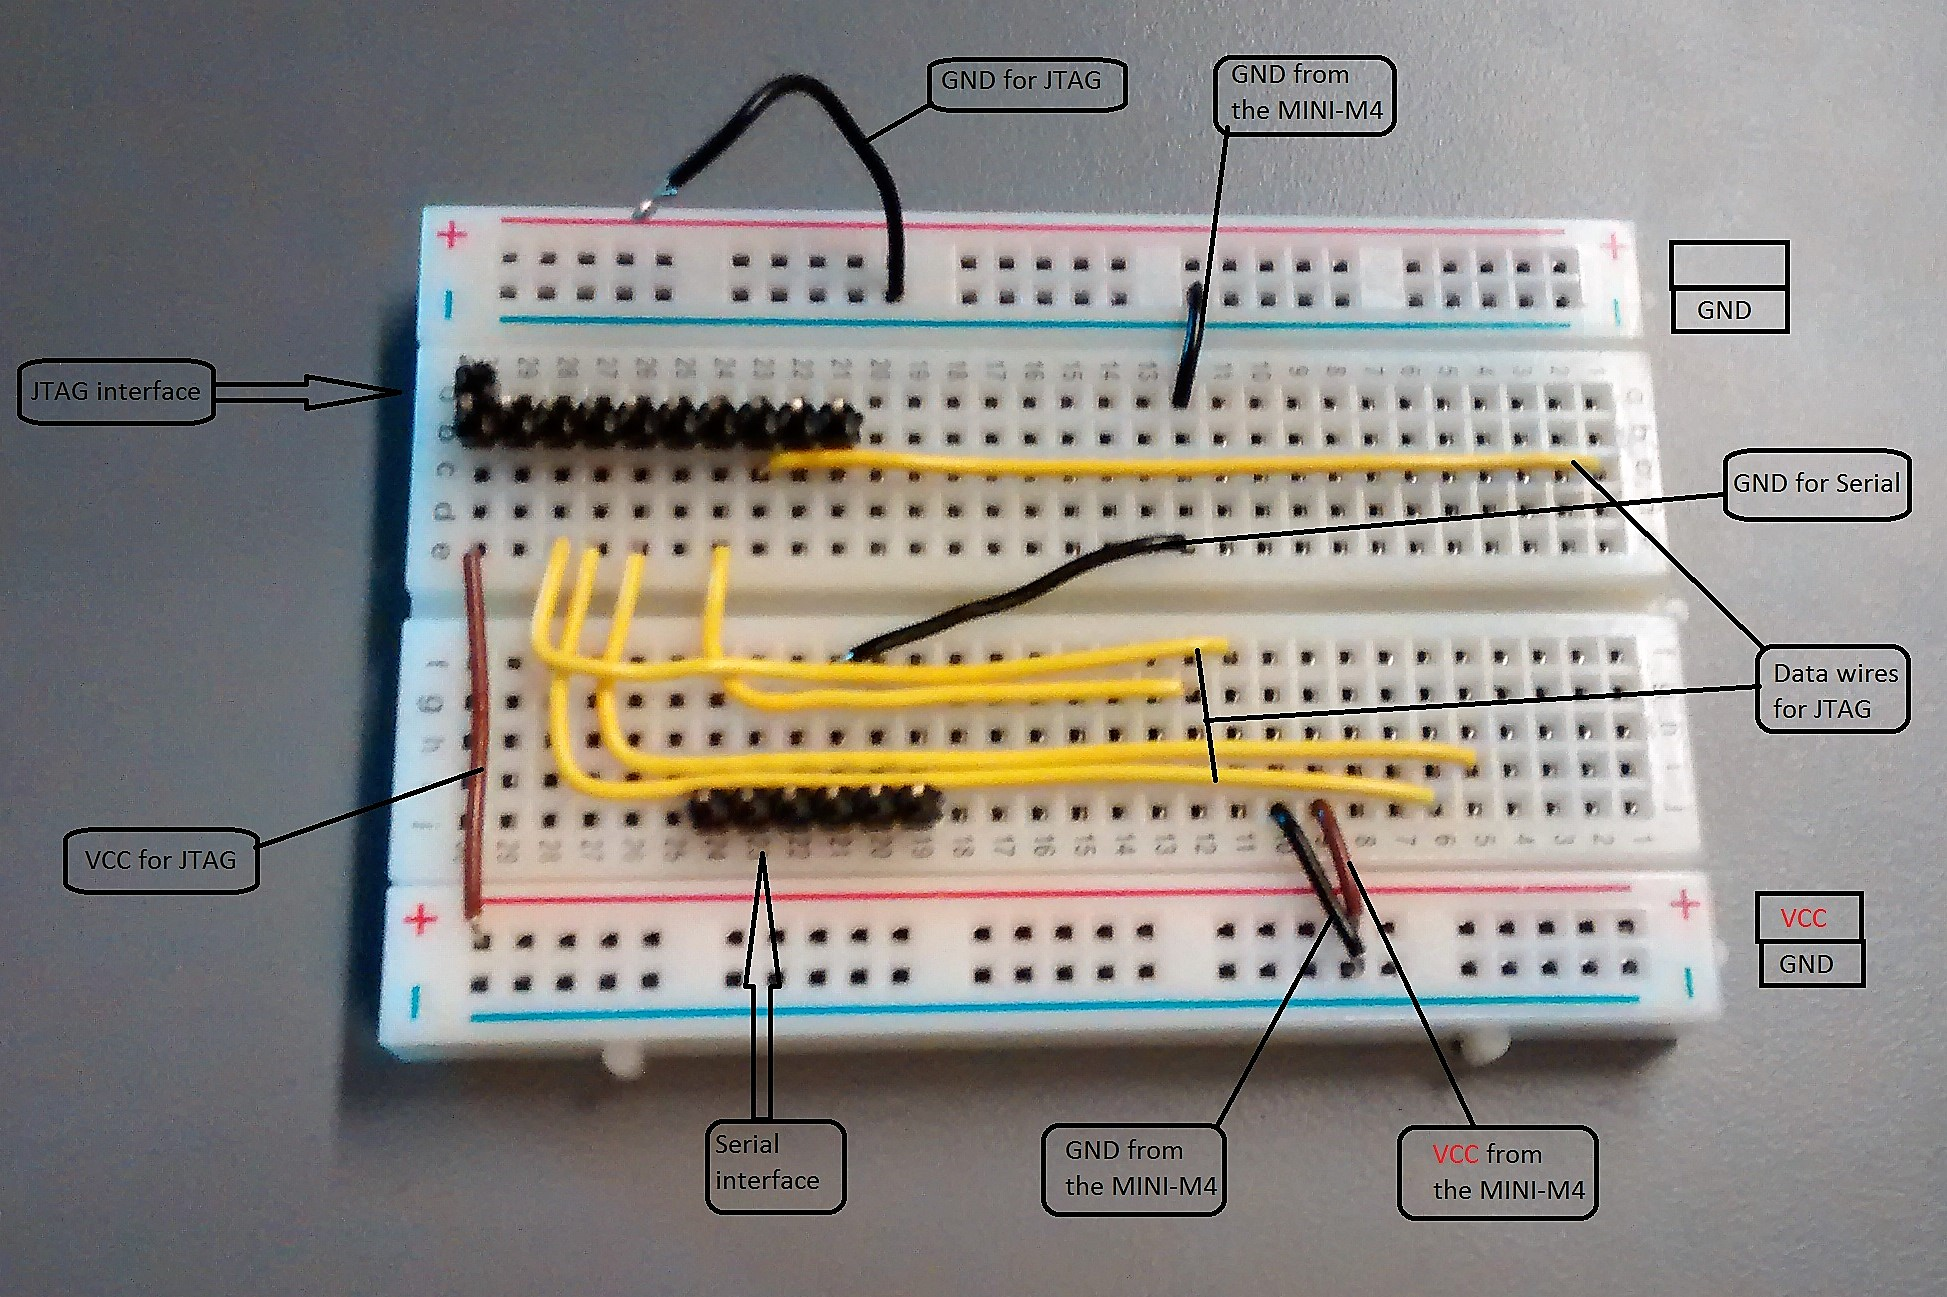
\includegraphics[width=\linewidth]{hardware/1_breadboard_only_edited}
\captionof{figure}{The wiring on the breadboard}
\label{figAPP:hardware_setup_1}
\end{figure}

Figure \ref{figAPP:hardware_setup_2}
shows the pinout of the JTAG connector. Out of the 20 pins, only
five will be used by the interface, and two for getting a voltage reference
into the module.
\begin{figure} [h]
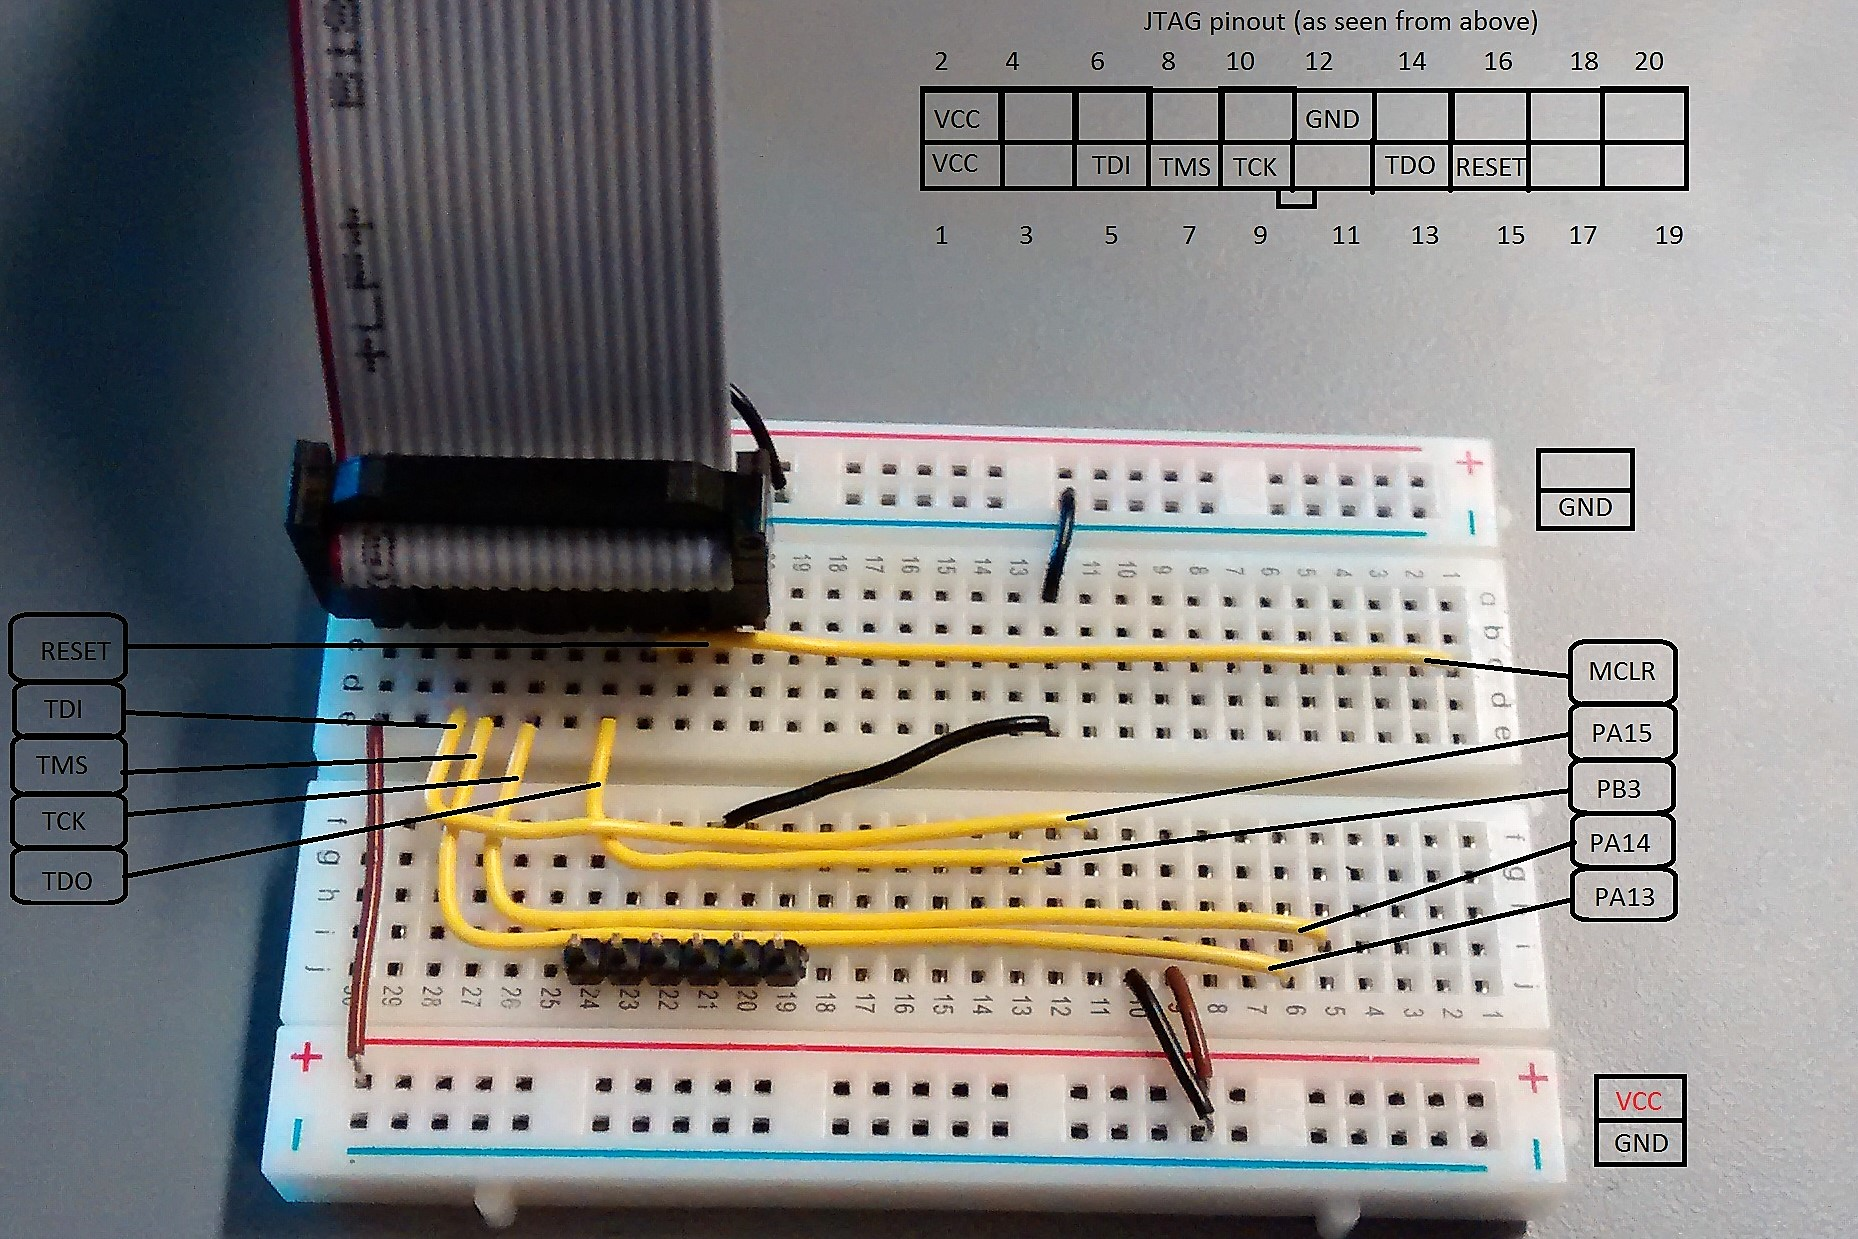
\includegraphics[width=\linewidth]{hardware/2_breadboard_jtag_edited}
\captionof{figure}{Breakout of the JTAG connector}
\label{figAPP:hardware_setup_2}
\end{figure}

Figure \ref{figAPP:hardware_setup_3}
shows the corresponding pins for the JTAG interface, on the Mini-M4
board. Some of the wires are hidden under the board.
\begin{figure} [H]
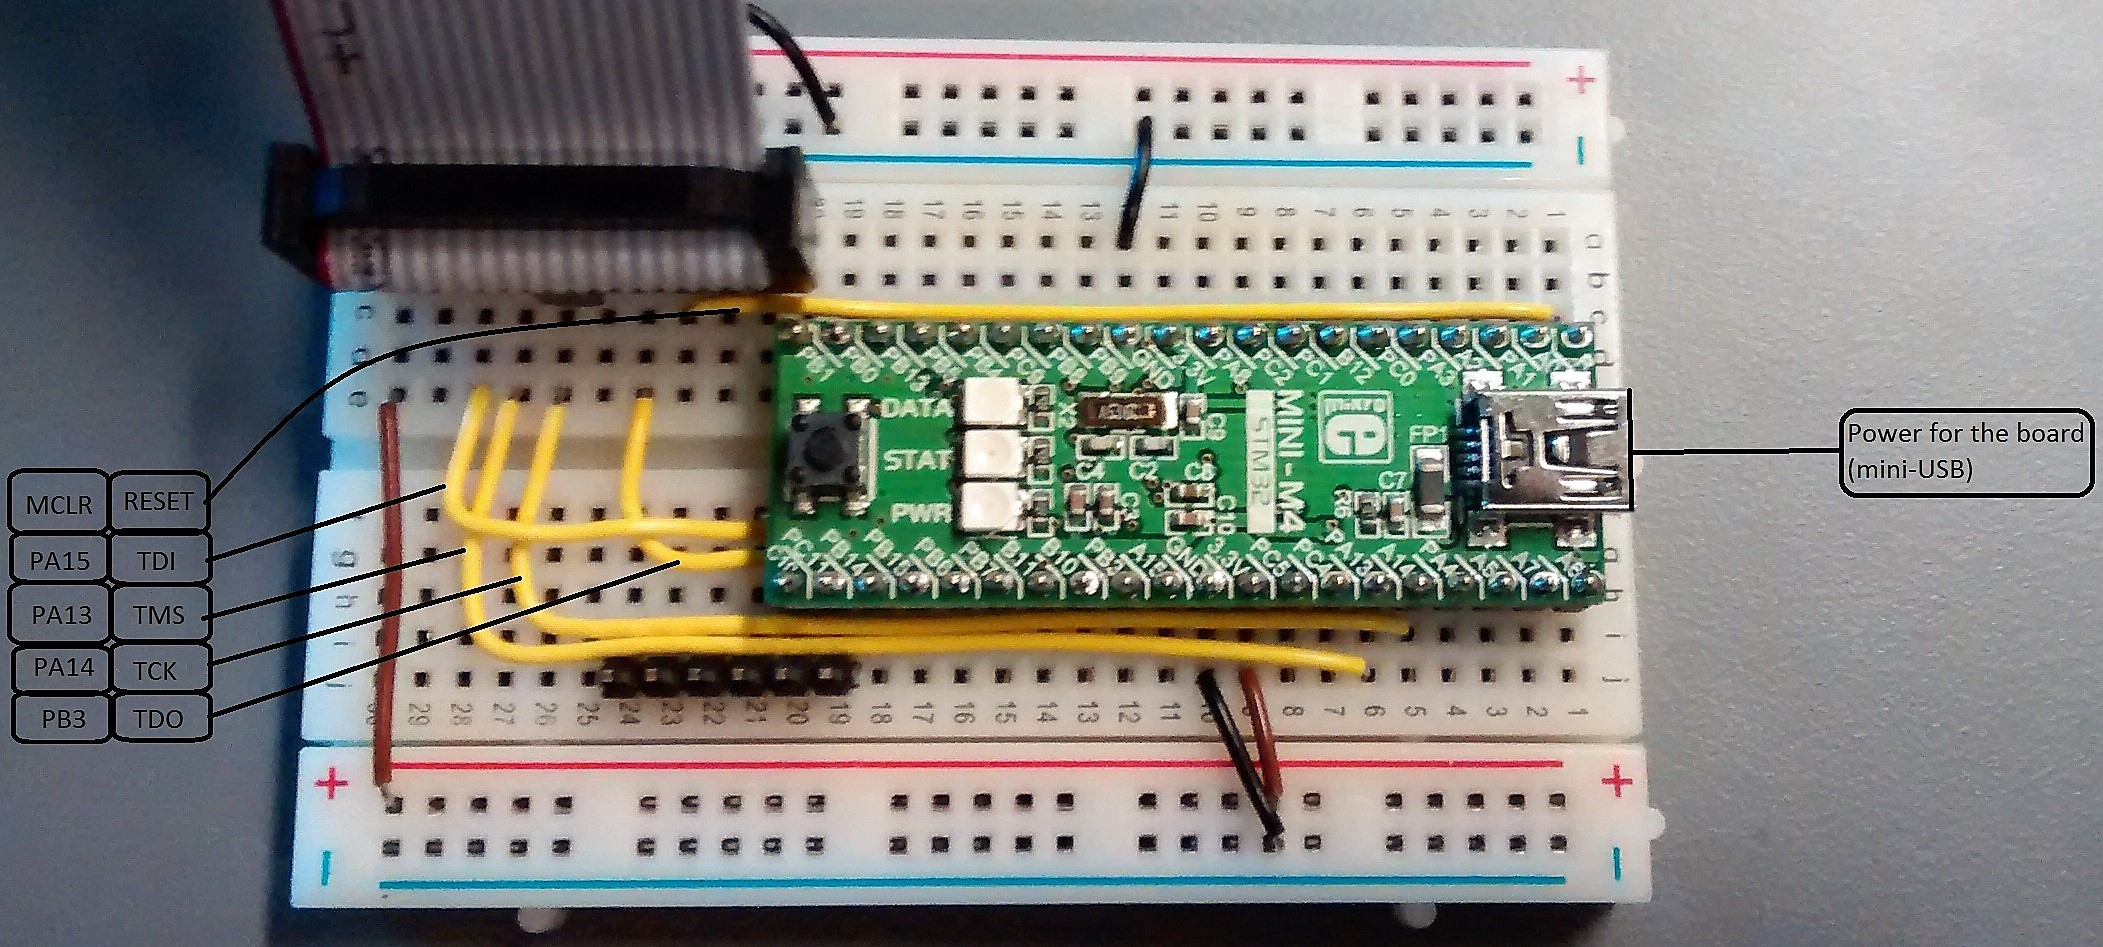
\includegraphics[width=\linewidth]{hardware/3_breadboard_mini_m4_edited}
\captionof{figure}{The five lines of the JTAG interface and their corresponding pins on the board}
\label{figAPP:hardware_setup_3}
\end{figure}

Figure \ref{figAPP:hardware_setup_4} 
shows the way the serial communication was connected. The only thing to
remember here is that the Tx of a device goes to the Rx of the 
other device it needs to communicate to.
\begin{figure} [h]
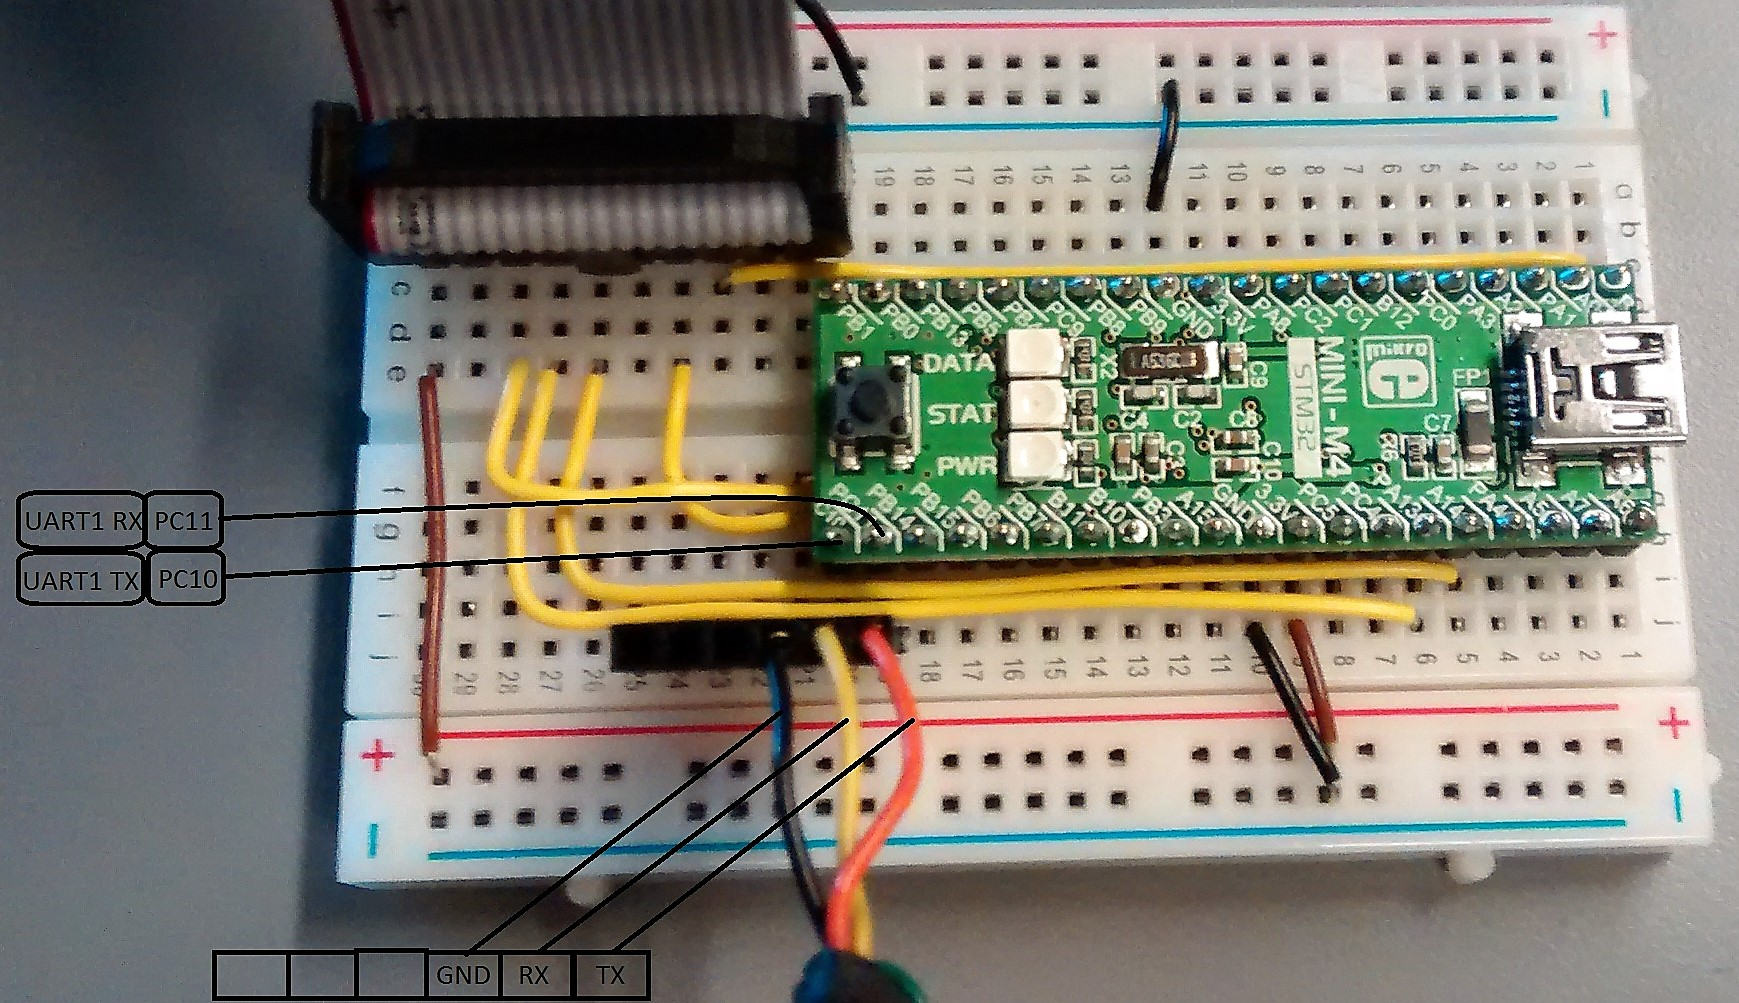
\includegraphics[width=\linewidth]{hardware/4_breadboard_mini_m4_serial_edited}
\captionof{figure}{Breakout of the serial communication}
\label{figAPP:hardware_setup_4}
\end{figure}